\documentclass[a4paper,12pt,oneside,oldfontcommands]{memoir}

% Castellano
% es-ucroman: evitar el warning por Fake sc para números romanos en minúscula
\usepackage[spanish,es-tabla,es-ucroman]{babel}
\selectlanguage{spanish}
\usepackage[utf8]{inputenc}
\usepackage[T1]{fontenc}
\usepackage{lmodern} % Scalable font
\usepackage{microtype}
\usepackage{placeins}
\usepackage{import}
\usepackage{float}
\usepackage{graphicx}


\RequirePackage{booktabs}
\RequirePackage[table]{xcolor}
\RequirePackage{xtab}
\RequirePackage{multirow}

% Links
\usepackage[colorlinks]{hyperref}
\hypersetup{
	allcolors = {blue}
}

% Ecuaciones y simbolos (tanto AMS como LaTeX
\usepackage{amsmath,amssymb,latexsym}

% Rutas de fichero / paquete
\newcommand{\ruta}[1]{{\sffamily #1}}

% Párrafos
\nonzeroparskip

% Huérfanas y viudas
\widowpenalty100000
\clubpenalty100000

% Paper size and margins (para A4)
\settrimmedsize{297mm}{210mm}{*}
\setlength{\trimtop}{0pt}
\setlength{\trimedge}{\stockwidth}
\addtolength{\trimedge}{-\paperwidth}
\settypeblocksize{634pt}{448.13pt}{*}
\setulmargins{4cm}{*}{*}
\setlrmarginsandblock{2.5cm}{2.5cm}{*}
\setmarginnotes{36pt}{36pt}{\onelineskip}
\setheadfoot{\onelineskip}{2\onelineskip}
\setheaderspaces{*}{2\onelineskip}{*}
\checkandfixthelayout

% Colores locales
\usepackage{xcolor}
\definecolor{ctitbox}{HTML}{E6E6FF}
\definecolor{capnum}{HTML}{0606FF}

% Imagenes
\usepackage{graphicx}
\newcommand{\imagen}[2]{
	\begin{figure}[!h]
		\centering
		\includegraphics[width=0.9\textwidth]{#1}
		\caption{#2}\label{fig:#1}
	\end{figure}
	\FloatBarrier
}

\newcommand{\imagenflotante}[2]{
	\begin{figure}%[!h]
		\centering
		\includegraphics[width=0.9\textwidth]{#1}
		\caption{#2}\label{fig:#1}
	\end{figure}
}


% El comando \figura nos permite insertar figuras comodamente, y utilizando
% siempre el mismo formato. Los parametros son:
% 1 -> Porcentaje del ancho de página que ocupará la figura (de 0 a 1)
% 2 --> Fichero de la imagen
% 3 --> Texto a pie de imagen
% 4 --> Etiqueta (label) para referencias
% 5 --> Opciones que queramos pasarle al \includegraphics
% 6 --> Opciones de posicionamiento a pasarle a \begin{figure}
\newcommand{\figuraConPosicion}[6]{%
  \setlength{\anchoFloat}{#1\textwidth}%
  \addtolength{\anchoFloat}{-4\fboxsep}%
  \setlength{\anchoFigura}{\anchoFloat}%
  \begin{figure}[#6]
    \begin{center}%
      \Ovalbox{%
        \begin{minipage}{\anchoFloat}%
          \begin{center}%
            \includegraphics[width=\anchoFigura,#5]{#2}%
            \caption{#3}%
            \label{#4}%
          \end{center}%
        \end{minipage}
      }%
    \end{center}%
  \end{figure}%
}

%
% Comando para incluir imágenes en formato apaisado (sin marco).
\newcommand{\figuraApaisadaSinMarco}[5]{%
  \begin{figure}%
    \begin{center}%
    \includegraphics[angle=90,height=#1\textheight,#5]{#2}%
    \caption{#3}%
    \label{#4}%
    \end{center}%
  \end{figure}%
}
% Para las tablas
\newcommand{\otoprule}{\midrule [\heavyrulewidth]}
%
% Nuevo comando para tablas pequeñas (menos de una página).
\newcommand{\tablaSmall}[5]{%
 \begin{table}
  \begin{center}
   \rowcolors {2}{gray!35}{}
   \begin{tabular}{#2}
    \toprule
    #4
    \otoprule
    #5
    \bottomrule
   \end{tabular}
   \caption{#1}
   \label{tabla:#3}
  \end{center}
 \end{table}
}

%
% Nuevo comando para tablas pequeñas (menos de una página).
\newcommand{\tablaSmallSinColores}[5]{%
 \begin{table}[H]
  \begin{center}
   \begin{tabular}{#2}
    \toprule
    #4
    \otoprule
    #5
    \bottomrule
   \end{tabular}
   \caption{#1}
   \label{tabla:#3}
  \end{center}
 \end{table}
}

\newcommand{\tablaApaisadaSmall}[5]{%
\begin{landscape}
  \begin{table}
   \begin{center}
    \rowcolors {2}{gray!35}{}
    \begin{tabular}{#2}
     \toprule
     #4
     \otoprule
     #5
     \bottomrule
    \end{tabular}
    \caption{#1}
    \label{tabla:#3}
   \end{center}
  \end{table}
\end{landscape}
}

%
% Nuevo comando para tablas grandes con cabecera y filas alternas coloreadas en gris.
\newcommand{\tabla}[6]{%
  \begin{center}
    \tablefirsthead{
      \toprule
      #5
      \otoprule
    }
    \tablehead{
      \multicolumn{#3}{l}{\small\sl continúa desde la página anterior}\\
      \toprule
      #5
      \otoprule
    }
    \tabletail{
      \hline
      \multicolumn{#3}{r}{\small\sl continúa en la página siguiente}\\
    }
    \tablelasttail{
      \hline
    }
    \bottomcaption{#1}
    \rowcolors {2}{gray!35}{}
    \begin{xtabular}{#2}
      #6
      \bottomrule
    \end{xtabular}
    \label{tabla:#4}
  \end{center}
}

%
% Nuevo comando para tablas grandes con cabecera.
\newcommand{\tablaSinColores}[6]{%
  \begin{center}
    \tablefirsthead{
      \toprule
      #5
      \otoprule
    }
    \tablehead{
      \multicolumn{#3}{l}{\small\sl continúa desde la página anterior}\\
      \toprule
      #5
      \otoprule
    }
    \tabletail{
      \hline
      \multicolumn{#3}{r}{\small\sl continúa en la página siguiente}\\
    }
    \tablelasttail{
      \hline
    }
    \bottomcaption{#1}
    \begin{xtabular}{#2}
      #6
      \bottomrule
    \end{xtabular}
    \label{tabla:#4}
  \end{center}
}

%
% Nuevo comando para tablas grandes sin cabecera.
\newcommand{\tablaSinCabecera}[5]{%
  \begin{center}
    \tablefirsthead{
      \toprule
    }
    \tablehead{
      \multicolumn{#3}{l}{\small\sl continúa desde la página anterior}\\
      \hline
    }
    \tabletail{
      \hline
      \multicolumn{#3}{r}{\small\sl continúa en la página siguiente}\\
    }
    \tablelasttail{
      \hline
    }
    \bottomcaption{#1}
  \begin{xtabular}{#2}
    #5
   \bottomrule
  \end{xtabular}
  \label{tabla:#4}
  \end{center}
}



\definecolor{cgoLight}{HTML}{EEEEEE}
\definecolor{cgoExtralight}{HTML}{FFFFFF}

%
% Nuevo comando para tablas grandes sin cabecera.
\newcommand{\tablaSinCabeceraConBandas}[5]{%
  \begin{center}
    \tablefirsthead{
      \toprule
    }
    \tablehead{
      \multicolumn{#3}{l}{\small\sl continúa desde la página anterior}\\
      \hline
    }
    \tabletail{
      \hline
      \multicolumn{#3}{r}{\small\sl continúa en la página siguiente}\\
    }
    \tablelasttail{
      \hline
    }
    \bottomcaption{#1}
    \rowcolors[]{1}{cgoExtralight}{cgoLight}

  \begin{xtabular}{#2}
    #5
   \bottomrule
  \end{xtabular}
  \label{tabla:#4}
  \end{center}
}


\graphicspath{ {./img/} }

% Capítulos
\chapterstyle{bianchi}
\newcommand{\capitulo}[2]{
	\setcounter{chapter}{#1}
	\setcounter{section}{0}
	\cleardoublepage\chapter*{{\color{blue} #1:} #2}
	\addcontentsline{toc}{chapter}{#1. #2}
	\markboth{#2}{#2}
}

% Apéndices
\renewcommand{\appendixname}{Apéndice}
\renewcommand*\cftappendixname{\appendixname}

\newcommand{\apendice}[1]{
	%\renewcommand{\thechapter}{A}
	\chapter{#1}
}

\renewcommand*\cftappendixname{\appendixname\ }

% Formato de portada
\makeatletter
\newcommand{\tutor}[1]{\def\@tutor{#1}}
\newcommand{\course}[1]{\def\@course{#1}}

%\usepackage{setspace}
\def\maketitle{
  \null
  \thispagestyle{empty}
  % Cabecera ----------------
    \begin{center}%
    	{\noindent\Huge \textsc{Universidad de Valladolid}}\\[.3cm]%
    	{\noindent\Large \textsc{Máster universitario}}\\[.3cm]%
    	{\noindent\Huge \textbf{Ingeniería Informática}}\\[1cm]%
    
    	
\includegraphics[height=3cm]{img/escudoUVA} \hfill
    	
\includegraphics[height=3cm]{img/escudoInfor.pdf} \hfill
    	\includegraphics[height=3cm]{img/escudoEIIVA.png} \hfill
    \end{center}%
  \vfill
    \begin{center}%
      % Título proyecto y escudo informática ----------------
      {\noindent\large\textsc{Trabajo Fin de Máster}}\\[.3cm]
      \colorbox{ctitbox}{%
        \begin{minipage}{.95\textwidth}
          \vspace{.2cm}\large
        %   \begin{center}
        %   \textsc{Máster en Ingeniería Informática}
        %   \end{center}
          \begin{center}
%          \renewcommand{\baselinestretch}{2.0}
          \textbf{\LARGE\@title{}}
%          \renewcommand{\baselinestretch}{1.0}
          \end{center}
          \vspace{.2cm}
        \end{minipage}
      }%
    \end{center}%
  \hfill
  \vfill
  % Datos de alumno, curso y tutores ------------------
  \begin{center}%
  {%
    \noindent\large
    Realizado por \Large\textbf{\@author{}}\\[0.2cm]
    \maltese\hspace{.1cm}\maltese\hspace{.1cm}\maltese\\[0.2cm]
    {\Large\sffamily\bfseries Universidad de Valladolid}\\
    \textbf{\@date{}}\\
    Tutor: \@tutor{}\\
  }%
  \end{center}%
  \null
  \cleardoublepage
}
\makeatother


% Evitar solapes en el header
\nouppercaseheads

% Datos de portada
\title{Comparación y evaluación de diferentes técnicas de IA para un modelo de rotación de empleados en empresas aplicado a equipos de fútbol}
\newcommand{\nombre}[0]{José María Lozano Olmedo} %%% cambio de comando
\newcommand{\depto}[0]{Departamento de Informática (ATC, CCIA, LSI)}
\newcommand{\areac}[0]{Lenguajes y Sistemas Informáticos}
\author{\nombre}
\tutor{Joaquín Adiego Rodríguez y Natalia Martín Cruz}
\date{\today}

\begin{document}

\maketitle


\newpage\null\thispagestyle{empty}\newpage


%%%%%%%%%%%%%%%%%%%%%%%%%%%%%%%%%%%%%%%%%%%%%%%%%%%%%%%%%%%%%%%%%%%%%%%%%%%%%%%%%%%%%%%%
\thispagestyle{empty}


\noindent
\begin{center}%
	{\noindent\Huge Universidad de Valladolid}\vspace{.5cm}%
	
\begin{center}%
	
\includegraphics[height=3cm]{img/escudoUVA} \hspace{1cm}
\end{center}%

	{\noindent\Large \textbf{Máster universitario en Ingeniería Informática}}\vspace{.5cm}%
\end{center}%



\noindent D. Joaquín Adiego Rodríguez, profesor del departamento de de Informática (ATC, CCIA, LSI), área de Lenguajes y Sistemas Informáticos y D. Natalia Martín Cruz, profesora del departamento de Organización de Empresas y CIM, área de Organización de Empresas.

\noindent \textbf{Expone}:

\noindent Que el alumno D. \nombre, %con DNI dni,
ha realizado el Trabajo final de Máster en Ingeniería Informática titulado "\makeatletter\textsc{\@title{}}\makeatother". 

\noindent Y que dicho trabajo ha sido realizado por el alumno bajo la dirección del que suscribe, en virtud de lo cual se autoriza su presentación y defensa.

\begin{center} %\large
En Valladolid, {\large \today}
\end{center}

\vfill\vfill\vfill



% Author and supervisor
\begin{minipage}{0.45\textwidth}
\begin{flushleft} %\large
Vº. Bº. del Tutor:\\[2cm]
D. Joaquín Adiego Rodríguez
\end{flushleft}
\end{minipage}
\hfill
\begin{minipage}{0.45\textwidth}
\begin{flushleft} %\large
Vº. Bº. del co-tutor:\\[2cm]
D. Natalia Martín Cruz
\end{flushleft}
\end{minipage}
\hfill

\vfill

% para casos con solo un tutor comentar lo anterior
% y descomentar lo siguiente
%Vº. Bº. del Tutor:\\[2cm]
%D. nombre tutor


\newpage\null\thispagestyle{empty}\newpage




\frontmatter

% Abstract en castellano
\renewcommand*\abstractname{Resumen}
\begin{abstract}
En los últimos años, la inteligencia artificial ha experimentado un exponencial crecimiento, revolucionando diferentes sectores con sus innovadoras ideas. Este crecimiento tecnológico no ha pasado desapercibido en el ámbito deportivo, donde la inteligencia artificial se está incorporando cada vez más para optimizar el rendimiento de los equipos y atletas. 

Este trabajo se centra en evaluar diversas técnicas de inteligencia artificial para predecir el rendimiento de equipos de fútbol mediante el análisis de la rotación de jugadores. El objetivo del proyecto es detectar cómo las diferentes estrategias de rotación aplicadas por los equipos afectan al desempeño del equipo y cómo la inteligencia artificial puede realizar predicciones en base a ellas para ayudar a optimizar estas estrategias y detectar cuáles son las mejores. Este trabajo abarca desde la recopilación y el análisis de datos asociados a las ligas seleccionadas, la creación de modelos de inteligencia artificial y la evaluación de su eficacia. Se pretende que con este proyecto se puedan obtener resultados significativos para optimizar la gestión de equipos de fútbol y así poder facilitar el trabajo a sus dirigentes.
\end{abstract}

\renewcommand*\abstractname{Descriptores}
\begin{abstract}
Fútbol, jugadores, inteligencia artificial, predicciones, rotación, rendimiento 
\end{abstract}

\clearpage

% Abstract en inglés
\renewcommand*\abstractname{Abstract}
\begin{abstract}
In recent years, artificial intelligence has experienced exponential growth, revolutionizing various sectors with its innovative ideas. This technological advancement has not gone unnoticed in the sports field, where artificial intelligence is increasingly being integrated to optimize team and athlete performance. 

This study focuses on evaluating various artificial intelligence techniques to predict the performance of football teams through the analysis of player rotation. The objective of the project is to detect how different rotation strategies applied by teams impact their performance, and how artificial intelligence can make predictions based on these strategies to optimize them and identify the best ones. This work ranges data collection and analysis from selected leagues, the development of artificial intelligence models, and the evaluation of their effectiveness. The goal is to achieve significant results with this project to optimize the management of football teams and thereby facilitate the work of their leaders.
\end{abstract}

\renewcommand*\abstractname{Keywords}
\begin{abstract}
Football, players, artificial intelligence, predictions, rotation, performance
\end{abstract}

\clearpage

% Indices
\tableofcontents
\clearpage
\listoffigures
\clearpage
\listoftables
\clearpage
\mainmatter

\capitulo{1}{Introducción}



\section{Contexto}
Este proyecto se desarrolla como el Trabajo de Fin de Máster del Máster en Ingeniería Informática No Presencial de la Escuela de Ingeniería Informática de la Universidad de Valladolid y como continuación del trabajo realizado durante la estancia en un GIR para la asignatura de I+D+i.

En los últimos años, el campo de la inteligencia artificial ha sufrido un crecimiento considerable, alterando diferentes aspectos de la sociedad moderna \cite{ia2}. En este contexto, el deporte, y en especial el fútbol, no se ha mantenido al margen. La capacidad de la inteligencia artificial para analizar grandes volúmenes de datos y extraer patrones útiles ha encontrado una aplicación cada vez más importante en el ámbito deportivo, proporcionando nuevas herramientas para optimizar el rendimiento de los equipos y la toma de decisiones por parte de los directivos y entrenadores \cite{ia1}.

El fútbol, es algo más que un simple juego, se ha convertido en un fenómeno global que supera todas las fronteras. Los clubes de fútbol son empresas con mucho dinero y todo lo relacionado con este deporte, de manera general, mueve grandes cantidades de dinero. En este contexto altamente competitivo, la presión por obtener resultados positivos es máxima, tanto en términos deportivos como financieros \cite{dinero}. 

Un claro ejemplo de esto es el fichaje de Neymar por el Paris Saint-Germain (PSG) en 2017, que se firmó por la desorbitada cantidad de 222 millones de euros. Este traspaso no solo rompió récords, sino que también destacó cómo los grandes clubes están dispuestos a invertir grandes cantidades para atraer a los mejores jugadores y a su vez, generar ingresos mediante la venta de camisetas, patrocinadores y entradas a los partidos. La presencia de estrellas de este nivel en los equipos aumenta el valor comercial de los clubes, atrayendo aún más patrocinadores, haciendo mejores los acuerdos de \textit{marketing} y por lo tanto mejorando el estado financiero de los equipos \cite{neymar}.

Por otro lado, los derechos de televisión son otra fuente crucial de ingresos en el fútbol. Las ligas más importantes, como la Premier League inglesa, reciben miles de millones de libras por la transmisión de sus partidos. Estos contratos televisivos proporcionan la capacidad a los clubes de repartir grandes sumas de dinero entre ellos, lo que permite financiar fichajes y salarios enormes. El torneo británico concedió sus derechos televisivos en la temporada 2022/2023 por todo el mundo por un valor total de 8.136 millones de libras \cite{premier-tv}.

Además, los estadios modernos se han convertido en auténticas obras de ingeniería. El Santiago Bernabéu del Real Madrid, por ejemplo, está siendo remodelado con una inversión cercana a los 1950 millones de euros. Esta obra no solo incrementará considerablemente la experiencia de los aficionados, sino que también permitirá al club generar ingresos adicionales a través de eventos no deportivos como conciertos y nuevas áreas comerciales, como ya está sucediendo. Así, el fútbol se está convirtiendo en una industria multimillonaria que atrae inversiones de todo el mundo, consolidándose como el principal espectáculo mundial \cite{bernabeu}.

En este escenario, la gestión eficiente de los recursos humanos, como en este caso los jugadores, se ha vuelto prioritaria para el éxito de un equipo. Los entrenadores y directivos se enfrentan al desafío de optimizar el rendimiento de sus jugadores tratando de minimizar el riesgo de lesiones y el cansancio físico. La inteligencia artificial ofrece herramientas potentes para abordar este desafío, permitiendo el análisis de datos relacionados con el estado físico de los jugadores, el rendimiento en partidos anteriores, las lesiones previas y otros factores relevantes.

La gestión de la rotación de jugadores es uno de los aspectos más críticos de la estrategia de un equipo a lo largo de una temporada y que tiene una mayor repercusión sobre su éxito (Mathew Hughes, Paul Hughes, Kamel Mellahi, Cherif Guermat, 2010 \cite{ingleses}) (Massaro, M., Mas, F.D., Bontis, N. and Gerrard, B., 2020 \cite{leeds}). La inteligencia artificial puede ayudar a los entrenadores a tomar decisiones documentadas sobre cuándo dar descanso a un jugador, cuándo alinear a un futbolista, qué cambios realizar y cómo mantener un equilibrio entre la competitividad y la salud de la plantilla. 

Los equipos de fútbol utilizan el análisis de datos para gestionar eficientemente a sus jugadores y optimizar su rendimiento en el campo, así como para reducir el riesgo de lesiones. Mediante tecnologías avanzadas y técnicas de última generación, los clubes recopilan un amplio campo de datos, incluyendo métricas de rendimiento físico como la distancia recorrida, velocidad, y cargas de trabajo. Estos datos permiten a los entrenadores y al personal médico controlar la condición física que tienen los jugadores en tiempo real, identificar patrones de fatiga, y ajustar los entrenamientos y tiempos de juego según como corresponda en base a los datos recopilados. 

Un club que aplica esto es el Liverpool FC que emplea el análisis de datos para tomar decisiones justificadas sobre cuándo rotar a sus jugadores, garantizando no sobrepasar sus límites físicos y que se mantengan al máximo rendimiento durante toda la temporada. Este enfoque basado en datos no solo aumenta el rendimiento individual y colectivo del equipo, sino que también ayuda a evitar lesiones, prolongando así la carrera de los jugadores y garantizando su disponibilidad y rendimiento para los partidos clave de la temporada donde es necesario que estén al 100\% \cite{liverpool}.

Por lo tanto, el uso de la inteligencia artificial en el fútbol no solo es una oportunidad para mejorar el rendimiento deportivo, sino también una necesidad para mejorar sobre los rivales en un entorno cada vez más competitivo y exigente. Los equipos que puedan lograr aprovechar e incorporar de manera efectiva estas herramientas tendrán una ventaja considerable sobre el resto para conseguir sus objetivos deportivos y financieros.

















\section{Motivación}

El crecimiento en los últimos años de la inteligencia artificial ha despertado un interés en su aplicación en diversos campos como en el deporte. En el ámbito del fútbol, la capacidad de utilizar la inteligencia artificial para analizar datos complejos y tomar decisiones estratégicas concretas en base a ellos, ofrece un gran potencial para incrementar el rendimiento de los equipos. Esta motivación se debe a la necesidad de los clubes por mantenerse competitivos en un entorno que está en constante evolución, donde la línea entre el éxito y el fracaso cada vez es más estrecha.

La inteligencia artificial ha transformado el ámbito deportivo al proporcionar herramientas avanzadas para el análisis de datos, la mejora del rendimiento y la toma de decisiones justificadas. En el fútbol, la inteligencia artificial se utiliza para analizar enormes volúmenes de datos de partidos, dando la capacidad a los entrenadores de desarrollar tácticas más precisas, adecuadas y adaptadas. Además, la inteligencia artificial optimiza la gestión de la salud de los deportistas al predecir el riesgo de lesiones y proponer programas de entrenamiento personalizados que se adapten a ellos. Fuera del campo, la inteligencia artificial cada vez mejora más la experiencia de los aficionados. La inteligencia artificial está revolucionando la forma en que los equipos y atletas se preparan y compiten, elevando el deporte de alto nivel a nuevos escalones \cite{ia-deporte}.

El proyecto aparece como respuesta al incremento en la demanda de herramientas que permitan a los clubes mejorar en la gestión de sus recursos humanos, en concreto de sus jugadores. La inteligencia artificial tiene la capacidad de analizar grandes cantidades de datos sobre los jugadores y equipos, detectando patrones y tendencias que pueden pasar desapercibidos para las personas. Al integrar estas conclusiones en la toma de decisiones, los equipos pueden mejorar la eficiencia de su rotación de jugadores, incrementando así sus posibilidades de éxito en el campo.

En los últimos años, la demanda de especialistas en análisis de datos en el ámbito deportivo ha aumentado considerablemente debido a la creciente importancia de los datos para optimizar el rendimiento y la estrategia de los equipos y atletas. Equipos y organizaciones deportivas ahora buscan analistas de datos para analizar métricas de rendimiento, evaluar riesgos de lesiones y desarrollar tácticas más eficientes contra sus rivales. Este crecimiento se debe a los avances tecnológicos y a la comprensión de que el análisis de datos puede generar una ventaja competitiva considerable, incrementando tanto el desempeño individual de los atletas como los resultados colectivos de los equipos \cite{incremento-ia-deporte}.

Este proyecto tiene el potencial para marcar un cambio significativo en la manera en que se realiza la gestión deportiva en el fútbol moderno. Al ofrecer a los clubes herramientas avanzadas de análisis y toma de decisiones, se espera que este proyecto ayude no solo a mejorar los resultados deportivos, sino también a fortalecer la posición competitiva y el rendimiento financiero de los equipos en un mercado cada vez más exigente y competitivo.













\section{Aplicaciones similares}
A continuación, se detallan aplicaciones y proyectos similares a lo que se pretende desarrollar y que pueden servir de referencia.
\begin{itemize}
\item \textbf{LaLiga Beyond Stats:}
esta es una iniciativa de LaLiga que tiene como objetivo emplear las últimas tecnologías, relacionadas con el análisis de datos y la inteligencia artificial, para proporcionar una comprensión más profunda y completa de los partidos. Esta plataforma busca ofrecer a los aficionados, entrenadores, jugadores y clubes herramientas innovadoras para analizar y entender el rendimiento en el fútbol, más allá de las estadísticas habituales, a través de datos en tiempo real y visualizaciones interactivas, proporcionando así un enfoque más inteligente y apasionado hacia el deporte \cite{beyondstats}.

\item \textbf{Aplicación de la inteligencia artificial en la Premier League:}
esta liga utiliza la inteligencia artificial para determinar las probabilidades de que un equipo gane un partido mediante el análisis de un amplio rango de datos. Estos factores abarcan datos históricos de partidos anteriores, como el rendimiento del equipo en casa y fuera de casa, su posición en la tabla de clasificación, su forma actual y lesiones de jugadores clave entre otros. Además, se tienen en cuenta variables más específicas, como la posesión de balón, los tiros a puerta, las oportunidades creadas y el rendimiento en defensa y en ataque. Estos datos son proporcionados a algoritmos de aprendizaje automático que son capaces de analizar patrones complejos y entrenar modelos predictivos que estiman las probabilidades de que gane el local, empaten o gane el visitante. De esta manera, la inteligencia artificial proporciona una herramienta útil para predecir resultados de partidos de fútbol con un alto grado de precisión, lo que puede ser utilizado por equipos, aficionados y casas de apuestas para tomar decisiones en base a diferentes argumentos \cite{oracle} \cite{iaFutbol}.

\item \textbf{Opta:}
es una empresa líder en análisis y datos deportivos que es capaz de proporcionar información detallada y estadísticas sobre una amplia gama de eventos deportivos, incluyendo fútbol, \textit{rugby}, \textit{cricket} y otros. Para ello, utiliza tecnologías avanzadas de recopilación y análisis de datos donde recopila datos en tiempo real durante los eventos deportivos y los convierte en información valiosa y estadísticas significativas que son utilizadas por equipos, entrenadores, medios de comunicación y aficionados para analizar de mejor manera el juego y evaluar el rendimiento de los jugadores y equipos. Opta se ha convertido en un recurso importantísimo en el mundo del deporte para análisis de datos y seguimiento de estadísticas \cite{opta}.

\item \textbf{Mejora del rendimiento de los jugadores mediante la ciencia de datos en el Liverpool FC:} como se ha comentado previamente, uno de los principales equipos y pioneros en este área que utiliza la ciencia de datos e inteligencia artificial para mejorar el rendimiento de sus jugadores es el Liverpool FC. Mediante un enfoque avanzado, emplean grandes cantidades de datos, incluyendo métricas de rendimiento físico, táctico y de salud, recogidos durante sus entrenamientos y partidos. Estos datos son analizados para mejorar las estrategias de juego, establecer entrenamientos personalizados y gestionar la carga de trabajo de los jugadores, lo que proporciona una gran ayuda a prevenir lesiones. Además, el análisis de datos permite al cuerpo técnico tomar decisiones razonadas sobre alineaciones y tácticas, ajustando su enfoque basándose en el rendimiento y las características del oponente, lo que contribuye considerablemente al éxito del equipo en la temporada.

\item \textbf{Aplicación móvil en Android que utiliza estimaciones econométricas para la predicción del ganador y el número de goles:} este trabajo (Gonzalo Herreros Diezhandino, 2020 \cite{tfg-ref}) consiste en una aplicación móvil que muestra datos de los partidos, próximos partidos por jugarse, alineaciones, clasificaciones y estadísticas de los equipos. Además junto a estos datos mediante estimaciones econométricas, utilizando distribuciones de Poisson para los goles de los equipos, muestra la probabilidad que tiene cada equipo de anotar un determinado número de goles o mediante distribuciones normales, para el ganador del partido muestra la probabilidad que existe de que el local gane el partido, de que termine en empate o de que gane el visitante. 

\end{itemize}
















\section{Estructura de la memoria}

Este documento se estructura de la siguiente forma:
\begin{description}

\item[Capítulo 2 Objetivos del proyecto:] en este capítulo se describen los objetivos que se quieren conseguir con la ejecución de este proyecto. Estos se dividen en dos categorías distintas,
los objetivos de desarrollo y los objetivos académicos.


\item[Capítulo 3 Conceptos teóricos:] en este capítulo se expone una explicación teórica de los conceptos más importantes que se han utilizado para el desarrollo de este proyecto.

\item[Capítulo 4 Técnicas y herramientas:] en este capítulo se describen las técnicas utilizadas para la obtención de los datos y las tecnologías utilizadas para el desarrollo del proyecto.


\item[Capítulo 5 Aspectos relevantes del desarrollo del proyecto:] en este capítulo se recogen los aspectos más interesantes del desarrollo del proyecto como los detalles sobre las fases de análisis, diseño e implementación y el tratamiento de los datos.


\item[Capítulo 6 Resultados:] en este capítulo se exponen los resultados obtenidos y todas las conclusiones que se han extraído en el desarrollo del proyecto y que pueden ayudar a los entrenadores a cómo gestionar los jugadores.


\item[Capítulo 7 Conclusiones y líneas de trabajo futuras:] en este capítulo se explican las conclusiones finales adquiridas del proyecto junto a las posibles líneas de trabajo futuras a seguir.

\item[Apéndice Manual de instalación:] en este apéndice se describe el repositorio donde se encuentra el código y cómo se puede instalar y desplegar.

\item[Apéndice Combinaciones de parámetros en los modelos de \textit{machine learning}:] en este apéndice se recogen las combinaciones de parámetros que se han evaluado al entrenar los modelos que utilizaban algoritmos de \textit{machine learning}.

\end{description}




\capitulo{2}{Objetivos del proyecto}

\section{Introducción}
En este capítulo se describen los objetivos que se pretenden conseguir con este proyecto, diferenciando entre objetivos de desarrollo y académicos.








\section{Objetivos de desarrollo}

\label{sec:desarrollo}
El principal objetivo de desarrollo es entrenar varios modelos con inteligencia artificial que ayuden a los entrenadores a tomar mejores decisiones sobre qué jugadores utilizar en un partido mediante los datos obtenidos en los partidos anteriores. Para ello, los principales objetivos de desarrollo para este proyecto son:
 \begin{enumerate}

    \item \textbf{Obtener los datos de los partidos de fútbol de varias ligas.}
    Para ello, mediante el \textit{scraping} se extraerán los datos de todos los partidos jugados en diferentes ligas y la información asociada a los jugadores.
    
    \item \textbf{Limpiar, transformar y analizar los datos obtenidos.}
    Se deberán limpiar y transformar los datos obtenidos para que puedan ser utilizados por los modelos que se pretenden crear. Además, se debe realizar un análisis previo sobre los datos para detectar posibles patrones.
    
    \item \textbf{Aplicar diferentes modelos de inteligencia artificial con los datos obtenidos.}
    En este punto, se debe evaluar el rendimiento que tienen los diferentes modelos sobre los datos obtenidos.

    \item \textbf{Optimizar el rendimiento de los modelos.}
    Después de entrenar los diferentes modelos sobre los datos, se debe realizar una optimización de sus parámetros para mejorar la precisión obtenida.

    \item \textbf{Seleccionar los mejores modelos y analizar su rendimiento proporcionado.}
    Sobre todos los modelos evaluados, se deberán seleccionar los que mejor se comporten y se deberá de analizar que calidad tienen.

    \item \textbf{Documentar los pasos seguidos en el proyecto.}
    Se deben documentar todos los pasos seguidos en el proyecto y justificar todas las decisiones tomadas incluyendo los objetivos, métodos y resultados de la investigación y desarrollo. Por otro lado se debe detallar la estructura, funcionamiento y uso del código.

    \item \textbf{Obtener conclusiones determinantes sobre qué estrategias son mejores.} Al finalizar el proyecto se deben obtener conclusiones que ayuden a los entrenadores a gestionar de mejor manera los jugadores y tras el desarrollo de este proyecto se debe justificar adecuadamente qué estrategias son las mejores.

 \end{enumerate}








 
\section{Objetivos académicos}
Estos objetivos se centran en seguir profundizando en los conocimientos aprendidos en diversas asignaturas de este Máster relacionadas con el \textit{Deep Learning} y el \textit{Big Data} y ponerlos en práctica en un proyecto completo. A continuación se detallan cada uno de estos objetivos:

\begin{enumerate}

    \item \textbf{Aplicar los conocimientos asociados a los pasos de extracción, transformación y carga de los datos.} Se pretende poner en práctica todos los conocimientos asociados al proceso de ETL \textit{(Extract, Transform and Load)} seguido en los proyectos de \textit{Big Data} para estructurar los datos y que puedan ser utilizados por los modelos.
    \item \textbf{Aplicar las técnicas aprendidas sobre modelos de inteligencia artificial y redes neuronales.} Se pretende seguir profundizando y aplicar los conocimientos adquiridos sobre redes neuronales e inteligencia artificial para que los modelos creados tengan la mayor precisión posible.
    
    \item \textbf{Aplicar las mejores prácticas aprendidas para crear gráficos para el análisis de los datos.} Se pretende realizar un análisis de los datos obtenidos para detectar patrones que puedan ayudar a los entrenadores en la toma de decisiones. En este análisis, se debe perseguir que los gráficos creados cumplan con las mejores prácticas que se han aprendido para la creación de interfaces gráficas para el análisis de datos.
    
 \end{enumerate}

\capitulo{3}{Conceptos teóricos}

\section{Introducción}


Las técnicas de inteligencia artificial abarcan una amplia gama de metodologías y enfoques. A continuación se detallan las técnicas más importantes que se han utilizado en este proyecto y sus conceptos teóricos.




\section{Introducción a la inteligencia artificial}

La Inteligencia Artificial (IA) es un campo de la informática que se dedica a la invención de sistemas que son capaces de realizar tareas que generalmente requieren capacidades humanas. Estas tareas abarcan desde el reconocimiento del habla, la toma de decisiones, la traducción de idiomas y el reconocimiento de patrones.

El término "Inteligencia Artificial" fue definido inicialmente por John McCarthy en 1956 durante la Conferencia de Dartmouth, que es conocido como el punto de partida del campo de la inteligencia artificial.

La IA ha revolucionado multiples industrias al proporcionar soluciones eficientes y precisas a problemas difíciles. Permite automatizar procesos, mejorar la toma de decisiones, personalizar experiencias de usuario y detectar patrones en enormes volúmenes de datos. Esto ha provocado mejoras significativas en productividad, innovación y calidad de vida y se aplica en diferentes áreas como la salud, finanzas, transporte y entretenimiento.

Las técnicas de inteligencia artificial se dividen en diversas áreas entre las que sobresalen el machine learning, deep learning, procesamiento del lenguaje natural, visión por computadora y sistemas de recomendación. A continuación, se definen las áreas que se utilizan en este proyecto.


\section{Machine learning}
El aprendizaje automático (Machine Learning) es considerada una subdisciplina de la inteligencia artificial que se dedica al desarrollo de algoritmos que permiten a las computadoras aprender a partir de datos y realizar predicciones o tomar decisiones sin haber sido programadas para llevar esas tareas. A continuación, se detallan los tipos que existen:
\begin{enumerate}
    \item \textbf{Aprendizaje supervisado:} aquí los algoritmos se entrenan con un conjunto de datos etiquetados, lo que quiere decir que cada ejemplo de entrenamiento está relacionado con una etiqueta. En este área destacan la regresión lineal y logistica, los árboles de decisión y bosques aleatorios y por último, las máquinas de vectores soporte.
    \item \textbf{Aprendizaje no supervisado:} en esta sección, los algoritmos trabajan con datos que no están etiquetados, y el objetivo es detectar patrones o estructuras ocultas en los datos. En este área destaca el algoritmo de Kmeans.
    \item \textbf{Aprendizaje por refuerzo:} finalmente, aquí los agentes aprenden a tomar decisiones al realizar una interacción con su entorno y reciben recompensas o castigos dependiendo de sus acciones. En este área destaca el algoritmo de Q-learning.
\end{enumerate}


En este proyecto principalmente se van a utilizar algoritmos de aprendizaje supervisado ya que el conjunto de datos esta etiquetado. En este proyecto se afronta un problema de clasificación porque a los datos se les asigna una de varias clases posibles, es decir, el objetivo es predecir la categoría o etiqueta correcta para cada dato entre múltiples clases predefinidas como puede ser el ganador del partido o el numero de goles.

Los algoritmos de este area asociados a problemas de clasificacion que se utilizan para entrenar los modelos en este proyecto con los datos obtenidos son los siguientes:
\begin{enumerate}
    \item \textbf{Árboles de decisión:} se encargar de dividir iterativamente el conjunto de datos en subconjuntos basados en las características más determinantes, estableciendo una estructura de árbol donde las hojas representan resultados de las decisiones y los nodos representan los atributos.
    \item \textbf{Máquinas de Vectores de Soporte (SVM):} es un algoritmo supervisado que encuentra el hiperplano óptimo que permite separar las clases en el espacio de características. Para problemas no lineales, SVM puede utilizar trucos de kernel para proyectar los datos a un espacio de una dimensión mayor donde las clases sean linealmente separables.
    \item \textbf{k-Vecinos Más Cercanos (k-NN):} k-NN es un algoritmo supervisado que permite predecir el valor de una nueva muestra en base a los k ejemplos más cercanos en el espacio de características. No contiene una fase de entrenamiento explícita, lo que lo hace simple y eficaz para conjuntos de datos pequeños.
    \item \textbf{Gradient Boosting Machines (GBM):} es un algoritmo supervisado que permite crear modelos predictivos a través de la construcción secuencial de árboles de decisión, donde cada árbol creado se encarga de corregir los errores del anterior. Los ejemplos más utilizados son XGBoost y LightGBM, que son bastante eficaces y permiten manejar grandes conjuntos de datos con alta dimensionalidad.
    \item \textbf{Random forest:} es un algoritmo supervisado que genera múltiples árboles de decisión entrenados en diversos subconjuntos del conjunto de datos y/o características. La predicción final la realiza mediante un proceso de agregación donde se utiliza la votación para clasificación, lo que incrementa la precisión y disminuye el sobreajuste. Destaca por ser robusto y eficaz para manejar conjuntos de datos grandes y complejos.
    \item \textbf{Gaussian Naive Bayes:} es un algoritmo de clasificación supervisada que se basa en el teorema de Bayes, que asume la independencia entre las características. A pesar de esta suposición en cierto modo simplificadora, es bastante eficaz y computacionalmente eficiente para problemas de clasificación de datos categóricos. 
\end{enumerate}


Se pueden utilizar diferentes métricas para evaluar los modelos entrenados con estos algoritmos sobre el conjunto de datos. Para este proyecto, a continuación, se detallan las principales métricas que se utilizan para evaluar los modelos creados:

\begin{enumerate}
    \item \textbf{Accuracy:} se define como la proporción de predicciones correctas entre el total de predicciones realizadas. Se calcula como (TP + TN) / (TP + TN + FP + FN), donde TP son los verdaderos positivos, TN son los verdaderos negativos, FP son los falsos positivos y FN son los falsos negativos. 
    \item \textbf{Precision:} se encarga de medir la proporción de verdaderos positivos entre las predicciones positivas. Se calcula como TP / (TP + FP). Determina la exactitud del clasificador al identificar verdaderos positivos, siendo fundamental en conjuntos de datos donde los falsos positivos tienen un alto valor.
    \item \textbf{Recall:} es la proporción de verdaderos positivos identificados correctamente entre todos los casos reales positivos considerados. Se calcula como TP / (TP + FN). Destaca su importancia en situaciones donde es crítico capturar todos los verdaderos positivos.
    \item \textbf{F1 Score:} es la media armónica entre la precisión y el recall, estableciendo un balance entre ambas métricas. Se calcula como 2 * (Precision * Recall) / (Precision + Recall). Es adecuada cuando se requiere un equilibrio entre precisión y recall.
    \item \textbf{Matriz de confusion:} es una tabla que ayuda a visualizar el rendimiento de un modelo de clasificación. Tiene cuatro cuadrantes: TP, TN, FP, y FN, que representan las verdaderas y falsas predicciones para las clases positivas y negativas que existen. Describe una visión detallada de cómo el modelo clasifica cada clase, ayudando a realizar el análisis de errores específicos de una clase.
\end{enumerate}





\section{Deep learning}
El aprendizaje profundo es una subdisciplina del aprendizaje automático que se dedica al uso de redes neuronales artificiales con varias capas profundas para modelar y comprender patrones complejos en los datos analizados. Se ha popularizado en los últimos años debido a su capacidad para superar a otros algoritmos en tareas como el reconocimiento de imágenes, procesamiento del lenguaje natural y otros campos. A continuación se detallan los componentes de la arquitectura de una red neuronal:

\begin{enumerate}
    \item \textbf{Neuronas artificiales:} simulan el funcionamiento de las neuronas biológicas. Cada neurona recibe varias entradas, las procesa mediante la denominada función de activación y produce una salida.
    \item \textbf{Capas:} las redes neuronales están compuestas por capas de neuronas. Las capas comunes incluyen la capa de entrada, capas ocultas y la capa de salida.
    \item \textbf{Funciones de activación:} introducen no linealidad en la red, dando la capacidad de que se modelen relaciones complejas. Ejemplos incluyen ReLU (Rectified Linear Unit), Sigmoide y Tanh.
\end{enumerate}

A continuacion se detallan los principales tipos de redes neuronales que existen:
\begin{enumerate}
    \item \textbf{Redes neuronales artificiales (ANN):} donde destaca el perceptrón multicapa, que  está compuesto por una capa de entrada, una o más capas ocultas y una capa de salida. Se entrena aplicando un proceso de retropropagación (backpropagation) y optimización. La backpropagation es un método de entrenamiento que se encarga de ajustar los pesos de las conexiones neuronales reduciendo el error entre las predicciones y los valores reales. Su tarea es calcular el gradiente del error con respecto a cada peso aplicando la regla de la cadena, propagando el error desde la salida hacia la entrada.
    \item \textbf{Redes neuronales convolucionales (CNN):} su arquitectura se divide en capas convolucionales que aplican filtros para extraer características locales de las imágenes, como pueden ser los bordes y texturas. Además incorpora capas de pooling que reducen la dimensionalidad de las características extraídas, manteniendo la información importante y disminuyendo el coste computacional. Finalmente, incorpora capas completamente conectadas que permiten conectar todas las neuronas de una capa a todas las neuronas de la siguiente capa, como en una ANN tradicional.
    \item \textbf{Redes neuronales recurrentes (RNN):} su arquitectura permite que la red contenga una memoria interna y sea capaz de procesar secuencias de datos al utilizar su salida como entrada en el siguiente paso temporal que va a realizar. En este caso destaca la LSTM que es una variante de la RNN diseñada para controlar dependencias a largo plazo mediante la incorporación de celdas de memoria y puertas de entrada, olvido y salida.

\end{enumerate}



En este caso, las principales métricas de evaluación para las redes neuronales coinciden con las de los modelos entrenados con algoritmos de machine learning.

Sin embargo, para las redes neuronales se utilizan algoritmos de optimización para ajustar los pesos de la red con el objetivo de minimizar la función de pérdida, incrementando así la precisión del modelo. El optimizador ayuda a la red a aprender patrones en los datos realizando iteraciones y ajustes incrementales. Los principales algoritmos de optimizacion para redes neuronales en problemas de clasificación son los siguientes:
\begin{enumerate}
    \item \textbf{Descenso de gradiente estocástico (SGD):} actualiza los pesos de la red neuronal usando el gradiente del error calculado en cada mini-lote de datos, realizando una actualización más frecuente y rápida pero que puede ser ruidosa. Sus ventajas son que es simple y eficiente para grandes conjuntos de datos.
    \item \textbf{Adam (Adaptive Moment Estimation):} junta las ventajas de AdaGrad y RMSProp, modificando las tasas de aprendizaje para cada parámetro en base a estimaciones de primer y segundo momento del gradiente. Sus ventajas son que es robusto y eficaz para problemas con grandes volúmenes de datos y alta dimensionalidad.
    \item \textbf{RMSProp (Root Mean Square Propagation):} ajusta la tasa de aprendizaje para cada parámetro de forma adaptativa, dividiendo el gradiente por la media móvil de magnitudes recientes de este gradiente. Es útil para manejar la tasa de aprendizaje en problemas donde los gradientes son cambiantes.
    
\end{enumerate}

Por otro lado, la función de pérdida de una red neuronal se utiliza para contar la discrepancia entre las predicciones del modelo y los valores reales. Se utiliza como guía para el ajuste de los pesos de la red durante el entrenamiento, colaborando a mejorar la precisión del modelo. Las principales funciones de pérdida para problemas de clasificacion que existen son:
\begin{enumerate}
    \item \textbf{Entropía cruzada (Cross-Entropy Loss):}
mide la discrepancia entre las distribuciones de probabilidad predicha y la real, penalizando considerablemente las predicciones incorrectas. Esta función de pérdida es ampliamente utilizada para problemas de clasificación binaria y multiclase, permitiendo ajustar las probabilidades predichas a las verdaderas.

\item \textbf{Categorical Cross-Entropy:}
es una forma específica de entropía cruzada que se utiliza en clasificación multiclase. Se calcula utilizando la probabilidad predicha para la clase verdadera y es habitual utilizarla en tareas de clasificación de imágenes y texto.

\item \textbf{Binary Cross-Entropy:}
similar a la entropía cruzada, pero específica solo para problemas de clasificación binaria. Calcula la pérdida como la media de las pérdidas individuales para cada clase binaria, penalizando las predicciones alejadas de las etiquetas binarias que realmente son verdaderas.

\item \textbf{Sparse Categorical Cross-Entropy:}
es una variante de la entropía cruzada categórica que se usa cuando las etiquetas están codificadas como enteros en lugar de vectores one-hot. Se utiliza para tareas de clasificación multiclase con muchas clases.
\end{enumerate}

Las épocas en una red neuronal determinan el número de veces que el algoritmo de entrenamiento procesa el conjunto completo de datos de entrenamiento. Cada época permite que la red ajuste sus pesos iterativamente para incrementar su rendimiento. Más épocas generalmente conducen a un mejor ajuste del modelo, aunque demasiadas pueden llevar al sobreajuste.

El batch size en una red neuronal se refiere al número de muestras de entrenamiento procesadas antes de actualizar los pesos del modelo. Establece la frecuencia con la que se ajustan los parámetros durante el entrenamiento. Un tamaño de lote más grande puede acelerar el entrenamiento, pero consume más recursos, mientras que un tamaño de lote menor puede realizar actualizaciones más precisas pero más lentas.

Los callbacks en una red neuronal son funciones personalizables que se activan en momentos específicos durante el entrenamiento, como al terminar cada época o cuando se alcanza cierta métrica. Permiten realizar acciones como guardar el modelo, reajustar la tasa de aprendizaje o parar el entrenamiento de forma temprana según ciertas condiciones. Los callbacks se utilizan para monitorear y mejorar el rendimiento del modelo durante el entrenamiento.

Ademas de todos aspectos, en la estructura de una red neuronal se pueden modificar los siguientes parámetros:
\begin{enumerate}
    \item \textbf{Dropout:}
es una técnica de regularización que desactiva aleatoriamente un porcentaje de neuronas durante el entrenamiento para evitar el sobreajuste, aumentando la capacidad de generalización del modelo.

\item \textbf{Batch Normalization:}
normaliza las activaciones de una capa antes de pasar a la siguiente capa, estabilizando y acelerando el proceso de entrenamiento al disminuir el cambio de variables internas.

\item \textbf{Bias Initializer y Regularizer:}
bias initializer establece cómo se inicializan los sesgos en las neuronas, mientras que el bias regularizer aplica una penalización para evitar el sobreajuste, haciendo que se mantengan los sesgos en valores razonables durante el entrenamiento.

\item \textbf{Kernel Initializer y Regularizer:}
kernel initializer establece cómo se inicializan los pesos de las neuronas, y el kernel regularizer aplica una penalización a los pesos para evitar el sobreajuste, permitiendo mantener los pesos del modelo bajo control.
\end{enumerate}

\section{Validacion cruzada y division de los datos}
Por otro lado, para el entrenamiento de los modelos se aplicará la técnica validación cruzada, que es un método de validación que divide el conjunto de datos en k subconjuntos y se encarga de entrenar el modelo k veces, cada vez con un subconjunto diferente cuyo objetivo es evaluar la capacidad del modelo para generalizar a datos no vistos.

Al entrenar los modelos, los datos se separan en un conjunto de entrenamiento, prueba y validacion. Dividir los datos en estos 3 conjuntos es crucial para evaluar y mejorar el rendimiento de un modelo. El conjunto de entrenamiento con un 70\% de los datos se utiliza para ajustar los parámetros del modelo, mientras que el conjunto de validación con un 15\% de los datos se emplea para ajustar los hiperparámetros y evitar el sobreajuste. Finalmente, el conjunto de prueba con un 15\% de los datos se utiliza para evaluar la capacidad de generalización del modelo a datos no vistos. Esta división permite asegurar que el modelo no solo se comporte bien con los datos conocidos sino que también sea efectivo con datos nuevos.



\capitulo{4}{Técnicas y herramientas}

\section{Introducción}
En este capítulo se detalla qué técnica se utiliza para la extracción de los datos y qué tecnologías se utilizan para el desarrollo del proyecto. 






\section{Obtención de los datos}
Para la obtención de los datos, se crean varios \textit{scripts} en Python que extraigan los datos de la página de Resultados De Fútbol \cite{resultadosfutbol} mediante \textit{scraping}.

El \textit{scraping} \cite{scraping} es una técnica utilizada para extraer automáticamente información de sitios web de forma automatizada. Consiste en el análisis y la recopilación de datos de páginas web. Estos programas acceden a la página web de la que se desean obtener los datos, identifican los componentes clave dentro del código HTML y extraen su información para su posterior procesamiento o análisis. El \textit{scraping} es una herramienta útil para obtener datos en gran volumen de manera rápida y eficiente y es aplicada en variedad de aplicaciones. En este proyecto se ha utilizado esta técnica para obtener los datos ya que no se ha podido encontrar ningún conjunto de datos que recoja información sobre los datos históricos de los partidos en las ligas seleccionadas. Además, mediante el \textit{scraping}, se puede fácilmente ir incorporando a los datos utilizados para crear los modelos los nuevos datos asociados a los últimos partidos jugados.





\section{Tecnologías utilizadas}

A continuación, se detallan las tecnologías base que se utilizan en el proyecto:


\begin{itemize}
  \item \textbf{Python:}
   es un lenguaje de programación versátil y de alto nivel que tiene una enorme popularidad en diversos campos, destacando en la ciencia de datos. Este lenguaje incorpora diferentes bibliotecas que permiten realizar diferentes tareas lo que le convierte en uno de los lenguajes con más funcionalidades diferentes \cite{python}. A continuación se detallan las principales bibliotecas de Python que se utilizan en este proyecto:
   \begin{itemize}
    \item \textbf{BeautifulSoup:} sirve para realizar tareas de \textit{scraping}. Esta biblioteca permite analizar y extraer datos de páginas web de manera sencilla y eficiente, ayudando al programador a realizar la manipulación de la estructura HTML de los sitios web para obtener la información que se desee sobre el sitio. Con BeautifulSoup, se pueden crear \textit{scripts} que naveguen por el contenido de una página web, identifiquen los elementos deseados y que permitan extraer datos de manera automatizada \cite{beautifulsoup}.
    \item \textbf{Scikit-learn:} Python es mundialmente utilizado en el campo de la inteligencia artificial y el \textit{machine learning} por bibliotecas como scikit-learn. Esta es una biblioteca que ofrece una diversa gama de herramientas para la creación de algoritmos de \textit{machine learning} como se pretende en este proyecto. Con scikit-learn, se pueden crear y entrenar modelos de \textit{machine learning} de forma eficiente, utilizando algoritmos ya definidos y técnicas avanzadas de análisis de datos \cite{scikit}.
    \item \textbf{Pandas:} facilita la manipulación y el análisis de datos estructurados mediante la introducción de los \textit{dataframes}. Estos son estructuras de datos bidimensionales que tienen la capacidad de almacenar y manipular datos de manera eficiente, de manera similar a una tabla de base de datos o una hoja de cálculo. Con pandas, se pueden cargar datos desde multitud de fuentes, realizar operaciones de limpieza y transformación de datos y realizar análisis estadísticos y exploratorios de manera rápida. Esto hace que pandas sea una herramienta indispensable para el almacenamiento y la manipulación de datos en proyectos de ciencia de datos y análisis de datos en Python como es en este caso \cite{pandas}.
   \end{itemize}
  
  \item \textbf{Keras:}
  es una API de alto nivel para la construcción, entrenamiento y evaluación de modelos de redes neuronales mediante Python. Destaca por su facilidad de uso y su enfoque en la creación rápida y sencilla de modelos de aprendizaje profundo facilitando el trabajo a los usuarios. Ofrece una sintaxis simple y fácil de entender y una abstracción de alto nivel que permite crear modelos complejos de manera rápida sin apenas esfuerzo, lo que lo convierte en una herramienta excelente que brinda flexibilidad y potente para trabajar en una amplia gama de proyectos de inteligencia artificial y aprendizaje profundo como es lo que se pretende en este caso. Esta tecnología se utiliza en este proyecto para crear modelos de redes neuronales que pueden tener un buen rendimiento sobre el conjunto de datos proporcionado \cite{keras}.

  \item \textbf{Tensorflow:}
  es una biblioteca de aprendizaje automático de código abierto que ha sido desarrollada por Google que proporciona una plataforma flexible y escalable para construir, entrenar y desplegar modelos de aprendizaje profundo con diversas características. Esta tecnología destaca por su capacidad para trabajar con grandes volúmenes de datos y su eficiencia en la ejecución en variedad de plataformas. TensorFlow ofrece una extensa gama de herramientas y funcionalidades, incluyendo la construcción de redes neuronales convolucionales, recurrentes y generativas, así como la experimentación con técnicas avanzadas. Por lo tanto, TensorFlow es una opción popular y extensamente utilizada para proyectos de inteligencia artificial y aprendizaje automático en diversas áreas. Esta tecnología se utiliza en este proyecto para la creación de modelos más avanzados que pueden tener un rendimiento elevado sobre los datos proporcionados \cite{tensorflow}.

  \item \textbf{Google Colaboratory:}
  es una plataforma gratuita de Jupyter Notebook que permite escribir y ejecutar código Python en el navegador. Está esencialmente diseñada para la enseñanza y la investigación en \textit{machine learning}, ya que proporciona acceso a grandes recursos de computación en la nube, incluyendo GPUs y memoria RAM. Colab también ayuda a la colaboración en tiempo real, permitiendo compartir y editar \textit{notebooks} entre diferentes usuarios. Además, se integra perfectamente con Google Drive para el almacenamiento y la gestión de archivos \cite{google-colab}.
  
  
  \end{itemize}

\capitulo{5}{Aspectos relevantes del desarrollo del proyecto}



\section{Introducción}
En este capitulo se recogen los aspectos más interesantes del desarrollo del proyecto, donde se documenta desde la metodologia aplicada para el desarrollo del proyecto, describiendo los pasos a seguir y el alcance que se espera que tenga el proyecto. Por otro lado, tambien se detalla la planificacion del proyecto, cual es el modelo de los datos, que operaciones de transformacion y limpieza han sido necesarias y finalmente se describe la implementacion de los archivos que forman parte del proyecto.


\section{Metodología}
La metodología de este proyecto tiene como base un enfoque que comprende varias etapas clave. En primer lugar, se realizará una revisión de diferentes artículos sobre técnicas de inteligencia artificial aplicadas al análisis de datos deportivos, centrándose especialmente en la predicción del rendimiento de equipos de fútbol basándose en la rotación de los jugadores. Esta revisión ayudará a identificar las mejores prácticas y los enfoques que pueden ser más relevantes para el desarrollo del proyecto.

Posteriormente, se llevará a cabo la recopilación y preparación de datos, donde se recogerán conjuntos de datos históricos que abarquen información relevante sobre la rotación de jugadores y el rendimiento deportivo de equipos de fútbol en las ligas seleccionadas. Esta etapa incluye la limpieza de datos, la preparación de los datos para su análisis posterior y un breve análisis sobre ellos para detectar patrones.

Una vez preparados los datos, se realizará la implementación y evaluación de modelos de inteligencia artificial. Se probarán los diferentes algoritmos comentados en la parte teorica y diferentes redes neuronales utilizando los parametros tambien comentados. Los modelos se entrenarán y ajustarán utilizando los datos que hemos obtenido previamente, y se evaluará su rendimiento utilizando kas métricas comentadas. Esta fase permitirá detectar los modelos más eficaces y precisos para predecir el rendimiento deportivo basado en la rotación de jugadores.

\section{Alcance}
El alcance de este proyecto abarca la evaluación y aplicación de diversas técnicas de inteligencia artificial para predecir el rendimiento de equipos de fútbol basándose en la rotación de jugadores. En primer lugar, se definirá la metodología y se seleccionarán las técnicas más correctas para el análisis de datos relacionados con la rotación de jugadores y el rendimiento deportivo. Este apartado incluirá la recopilación, preprocesamiento y análisis de los datos de las ligas, equipos y jugadores de fútbol seleccionados. Para la parte del análisis de los datos, se realizan unos pequeños programas que analicen los datos obtenidos mediante mapas de calor para poder detectar patrones. Al detectar estos patrones se pretende justificar si las estrategias de rotacion aplicadas por los equipos mejoran el rendimiento o no.

Las ligas sobre las que se obtendrán y utilizarán los datos serán LaLiga EA Sports (primera división española), Premier League (primera división inglesa) y Bundesliga (primera división alemana) desde la temporada 2018/2019 hasta la temporada 2023/2024, ambas incluidas.

Además, el alcance del proyecto se pretende que también implique la implementación y ajuste de modelos de inteligencia artificial para la predicción del rendimiento deportivo en función de la rotación de jugadores. Para ello, se explorarán diversas técnicas de inteligencia artificial y \textit{machine learning}, como redes neuronales, árboles de decisión, y métodos de aprendizaje automático supervisado y no supervisado, con el objetivo de detectar aquellas que mejor se adapten a las características de este problema. Sobre cada una de ellas, se realizará una optimización de parámetros para mejorar todo lo posible su precisión.
Finalmente, se realizará una evaluación de los modelos desarrollados, utilizando métricas de rendimiento para definir su eficacia y precisión en la predicción del rendimiento de los equipos. Después de esto, se seleccionará el mejor modelo y se evaluará su rendimiento en la actualidad aplicándolo sobre partidos que estén por jugarse.

Además de todos estos aspectos comentados, se documentarán y analizarán todas las tareas realizadas en el proyecto, con el objetivo de ofrecer recomendaciones para la gestión de la rotación de jugadores en equipos de fútbol, así como posibles áreas de mejora y futuras investigaciones para este proyecto.




\section{Plan de proyecto}

El proyecto comienza las primeras semanas durante la estancia en un GIR para la asignatura de I+D+i donde se realiza una parte de investigacion y se desarrolla el nucleo del proyecto. Para finalizar, el proyecto continua como Trabajo de Fin de Master, donde se sigue profundizando y expandiendo el trabajo realizado previamente. La duracion de cada una de estas secciones es 190 horas y 150 horas respectivamente, sumando en total 340 horas. La fecha de inicio del proyecto es el 29 de abril de 2024 y la fecha limite de finalizacion es el 28 de junio de 2024.


La Tabla \ref{table:planificacion} muestra la planificación de las semanas durante las que se desarrolla el proyecto.

\begin{table}[]
  \centering
  \begin{tabular}{|c|c|c|c|c|}
  \hline
  { \textbf{Semana}} & { \textbf{Fecha de inicio}} & { \textbf{Fecha de fin}} & { \textbf{Carga de trabajo}}& { \textbf{Sección}} \\ \hline
  1 & 29/04/2024 & 05/05/2024 & 40 horas  & I+D+i                                              \\ \hline
  2 & 06/05/2024 & 12/05/2024 & 40 horas   & I+D+i                                         \\ \hline
  3 & 13/05/2024 & 19/05/2024 & 40 horas   & I+D+i                                             \\ \hline
  4 & 20/05/2024 & 26/05/2024 & 30 horas   & I+D+i                                              \\ \hline
  5 & 27/05/2024 & 02/06/2024 & 24 horas   & I+D+i                                         \\ \hline
  6 & 03/06/2024 & 09/06/2024 & 16 horas    & I+D+i                                               \\ \hline
  7 & 10/06/2024 & 16/06/2024 & 60 horas    & TFM                                             \\ \hline
  8 & 17/06/2024 & 23/06/2024 & 60 horas    & TFM                                           \\ \hline
  9 & 24/06/2024 & 28/06/2024 & 30 horas   & TFM                                            \\ \hline
  \end{tabular}
  \caption{Planificación de las semanas.}
\label{table:planificacion}
  \end{table}

\section{Modelo de los datos}
Los datos obtenidos se asocian a diferentes entidades que estan relacionadas entre si y abarcan multitud de campos, por ello, es importante estructurarlos de la manera correcta para que lpuedan ser utilizados adecuadamente en el entrenamiento de los modelos. En la figura \ref{fig:arquitectura-logica} se puede apreciar el modelo de los datos y como se han almacenado de forma estructurada despues de extraerlos mediante scraping.



A continuacion, se realiza una breve descripcion de cada entidad:

\section{Limpieza y transformación de los datos}
Las tareas de limpieza y transformacion de los datos para prepararlos para que puedan ser utilizados en el entrenamiento de los modelos se describen a continuacion:

\begin{itemize}
    \item \textbf{Eliminar datos sobre substituciones de jugadores no detectados:} se han eliminado los registros de datosJugadoresPartidos donde no se ha podido extraer la posicion sobre el jugador sustituido. Esto ha sucedido un con apenas 3 jugadores en todas las ligas y temporadas evaluadas y por lo tanto el numero de registros afectados en minimo.
    \item \textbf{Seleccionar partidos a partir de la jornada 10:} se han filtrado los datos de los partidos dejando solamente los partidos jugados desde la jornada 10 hasta el final. Esto se ha hecho ya que los datos que se tienen en cuenta para cada partido unicamente consideran los partidos previos de los equipo que disputan ese encuentro en esa temporada y por tanto, hasta la jornada 10, no se considera que existen datos suficientes para obtener conclusiones estables sobre como se comporta ese equipo.
    \item \textbf{Eliminacion de ids:} para preparar los datos para entrenar los modelos, se han eliminado tanto el id del partido asociado como el id unico del dato para cada registro con los datos de los indicadores para un partido.
    \item \textbf{Transformacion de la clase:} antes de entrenar las redes neuronales con los datos obtenidos, se han transformado los datos de los registros de la clase a predecir, ya sea el ganador del partido, el numero de goles del local o el numero de goles del visitante, aplicando one-hot para que las redes neuronales puedan utilizar estos datos.
    \item \textbf{Normalizacion de los datos:} esta es una técnica de preprocesamiento que ajusta los valores de los datos para que se encuentren en un rango común que en este caso es [0, 1]. Esto mejora la eficiencia y la precisión de los algoritmos de machine learning al garantizar que todas las características contribuyan equitativamente. En este caso, es crucial para evitar que características con valores más grandes dominen el modelo ya que hay atributos que pueden tomar valores muy grandes y otros valores muy pequeños.
    
\end{itemize}


\section{Implementación}
El codigo del proyecto se ha ejecutado en una maquina virtual proporcionada por la Escuela
Todo el codigo del proyecto se ha dividido en diferentes carpetas. A continuacion se detalla la finalidad de cada una estas carpetas y sus archivos:
\capitulo{6}{Resultados y conclusiones obtenidas sobre los datos}

\section{Introducción}
En este capítulo se detallan los resultados y conclusiones que se han podido obtener de los datos y de los modelos creados para así poder determinar cuáles son las mejores estrategias de rotación de jugadores y así poder definir conclusiones claras que puedan ayudar a los entrenadores y directivos a tomar decisiones. 

\section{Conclusiones extraídas del análisis previo de los datos}

Previo al entrenamiento de los modelos, se ha realizado un análisis de los datos obtenidos para 
extraer posibles patrones sobre ellos y obtener conclusiones que puedan ayudar a los entrenadores a la hora de la toma de decisiones. Para realizar esto, se ha extraído el valor de cada indicador 
analizado de forma general para cada equipo en el último partido de la temporada que jugase y 
después se ha realizado la clasificación ordenando de mayor a menor por este indicador entre 
todos los equipos de esa liga. Después se ha evaluado en cuantas posiciones difiere la posición de 
este equipo en esta clasificación por el indicador respecto a la clasificación original ordenando 
por puntos. 

Con estos datos, se ha realizado un mapa de calor de manera que las diferencias negativas se 
marcasen en rojo y las diferencias positivas se marcasen en verde. Mediante este análisis se 
pretenden desmentir o confirmar pensamientos que están extendidos de forma generalizada en el 
mundo de fútbol y que pueden ayudar a extraer conclusiones de los datos, como por ejemplo, los 
equipos que hacen más cambios introduciendo delanteros, anotan más goles. A continuación, se detalla un ejemplo de cómo se explica y analiza este mapa de calor.

En la Figura \ref{fig:explicacion-mapa} se muestran los datos para los equipos de LaLiga en la temporada 2024 para 
la proporción de cambios en la alineación de delanteros en sus partidos en general.

\begin{figure}[H]
    \centering
    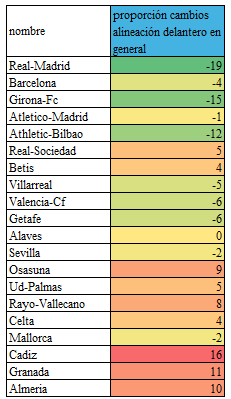
\includegraphics[scale=0.75]{svg/explicacion-tabla.png}
    \caption{Explicación sobre el mapa de calor para las diferencias de posiciones de clasificación. }
    \label{fig:explicacion-mapa}
\end{figure}



Aquí se puede observar que el Real Madrid tiene un valor de -19 en verde. Esto se explica porque 
hay 19 posiciones de diferencia entre su posición por la clasificación por puntos y su posición en 
la clasificación por este indicador que es la proporción de cambios en la alineación de delanteros 
en sus partidos en general. Por lo tanto, es un equipo con alto rendimiento ya que ocupa posiciones 
altas en la clasificación por puntos, pero sin embargo no suele realizar muchos cambios de 
delanteros en sus alineaciones iniciales. Por el contrario, el Cádiz que tiene un valor de 16 en rojo, 
se debe a que ocupa una baja posición en la clasificación por puntos, pero por otro lado, ocupa 
una alta posición en la clasificación por este indicador. Por lo tanto, es un equipo que tiene pocos 
puntos y un bajo rendimiento y que tiene una elevada proporción de cambios de delanteros en su 
alineación inicial.

En conclusión, en el análisis de este indicador se aprecia que los equipos de la zona alta de la 
clasificación por puntos tienen valores bajos en la proporción de cambios de delanteros en la 
alineación inicial y los equipos de la zona baja de la clasificación por puntos tienen valores altos 
en la proporción de cambios de delanteros en la alineación inicial.

A continuación, se detallan el resto de las principales conclusiones extraídas que se han podido 
apreciar de manera generalizada en todas las temporadas de las ligas evaluadas mediante este 
análisis:


\begin{itemize}
    \item Los equipos que realizan más cambios en las alineaciones iniciales entre un partido y otro
    tienden a estar en las posiciones más bajas de la clasificación y por el contrario, los 
    equipos que realizan menos cambios en las alineaciones iniciales entre un partido y otro, 
    tienden a estar en las posiciones más altas de la clasificación. Este efecto se aprecia sobre 
    todo si los cambios en las alineaciones iniciales afectan a los defensas o delanteros.
    \item Los equipos que realizan más cambios antes del descanso tienden a estar en posiciones 
    más bajas en la clasificación. Esto se puede apreciar sobre todo en la Premier League y 
    Bundesliga. Por otro lado, para todas las ligas, los equipos que hacen menos cambios 
    entre los minutos 61 a 75, tienden a ocupar posiciones más altas en la clasificación.
    \item Los equipos que hacen más cambios sacando defensas e introduciendo jugadores más
    ofensivos, suelen ocupar posiciones más bajas en la clasificación. Por otra parte, los 
    equipos que hacen menos cambios sacando delanteros e introduciendo jugadores más
    defensivos, tienden a ocupar posiciones más altas en la clasificación.
    \item Respecto a la media de los minutos en la que los equipos realizan los cambios, los equipos 
    de la zona alta de la clasificación tienen valores más bajos en este valor, por lo tanto, de 
    media suelen realizar los cambios antes.
    \item Los equipos de la zona alta de la clasificación suelen hacer menos cambios de jugadores 
    que han sido amonestados con amarilla.
    \item Finalmente, los equipos de la zona alta de la clasificación suelen tener menores valores en la 
    proporción de cambios que realizan por partido, es decir, en sus partidos no suelen gastar
    los 5 cambios de los que disponen.
    
\end{itemize}

El mapa de calor global agrupando todos los datos de los equipos en las ligas y temporadas consideradas para todos los indicadores analizados se puede ver a continuación en las Figuras \ref{fig:primera-calor}, \ref{fig:segunda-calor} y \ref{fig:tercera-calor}. Sin embargo, es importante detallar los siguientes aspectos sobre estos mapas de calor.
\begin{itemize}
    \item Solo se muestran los datos de las primeras cinco posiciones y de las últimas cinco. En el caso de las últimas cinco se utiliza esa nomenclatura de ultima, penúltima... ya que la Bundesliga tiene menos equipos y por tanto el último de su clasificación ocupa la posición 18 y no la 20 como sucede en LaLiga y la Premier League. Por lo tanto, la última posición, para todas las ligas, se corresponde con el equipo que ocupa la última posición, ya sea la 20 en ligas de 20 equipos (LaLiga y Premier League) o la 18 en la Bundesliga.
    \item Cada valor de este mapa de calor global se calcula mediante el promedio de cada valor en esa posición de los datos de cada liga y temporada analizada. Por lo tanto, los datos que se ven en las Figuras \ref{fig:primera-calor}, \ref{fig:segunda-calor} y \ref{fig:tercera-calor}, se obtienen al hallar el promedio de las diferencias de posiciones para cada una de las diez posiciones que se muestran con los datos de las diferentes ligas y temporadas evaluadas. Por ejemplo, para la primera posición del indicador porcentaje de cambios de defensas a centrocampistas, el valor se ha obtenido calculando el promedio con los valores asociados a la diferencia de clasificación del equipo que acabó en primera posición en la clasificación por puntos en cada una de las temporadas y ligas evaluadas para ese indicador. 
\end{itemize}

\begin{figure}[H]
    \centering
    \rotatebox{90}{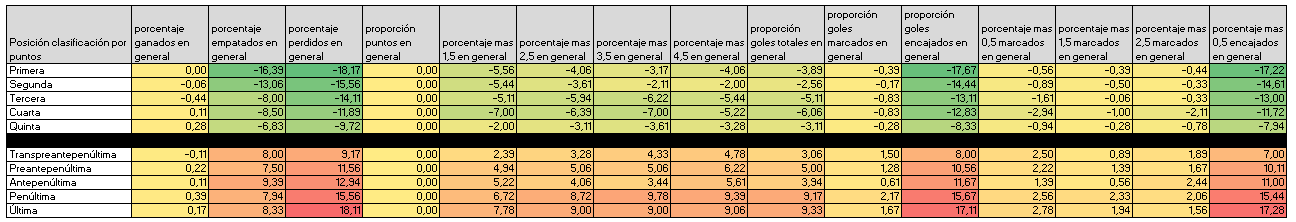
\includegraphics[scale=0.60]{svg/mapa-calor1.png}}
    \caption{Primera parte del mapa de calor global con las diferencias de posiciones de clasificación. }
    \label{fig:primera-calor}
\end{figure}

\begin{figure}[H]
    \centering
    \rotatebox{90}{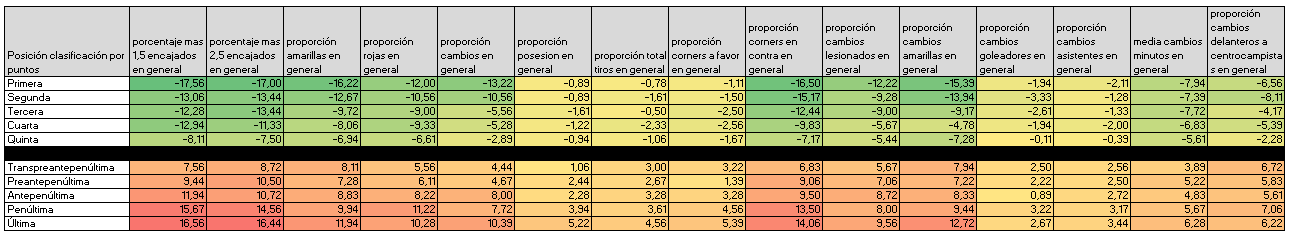
\includegraphics[scale=0.60]{svg/mapa-calor2.png}}
    \caption{Segunda parte del mapa de calor global con las diferencias de posiciones de clasificación. }
    \label{fig:segunda-calor}
\end{figure}

\begin{figure}[H]
    \centering
    \rotatebox{90}{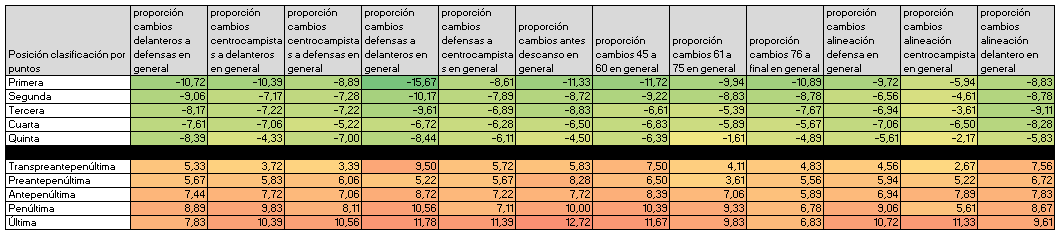
\includegraphics[scale=0.60]{svg/mapa-calor3.png}}
    \caption{Tercera parte del mapa de calor global con las diferencias de posiciones de clasificación. }
    \label{fig:tercera-calor}
\end{figure}












\section{Conclusiones extraídas al entrenar los modelos}




Se ha podido observar que en las predicciones realizadas por el modelo para predecir el ganador 
del partido, las variables que más repercusión tienen para aumentar la probabilidad de victoria del
equipo local son la proporción de este equipo de realizar cambios entre los minutos 61 a 75, la
proporción de cambios de defensas a centrocampistas y la proporción de cambios de
centrocampistas a defensas y para el visitante la proporción de este equipo de cambios de
centrocampistas a defensas, la proporción de cambios de defensas a delanteros y la proporción de 
cambios entre el minuto 76 al final. Los equipos con valores más elevados en estos indicadores 
tienen según el modelo más probabilidad de ganar el partido.

Por otro lado, para el modelo que predice la probabilidad que tiene el equipo local de marcar un 
determinado número de goles, las variables que tienen más repercusión para aumentar las 
probabilidades de que el equipo marque más goles son la proporción de este equipo de cambios 
entre los minutos del 45 al 60, la proporción de cambios de defensas a centrocampistas, la 
proporción de cambios de defensas a delanteros y la proporción de cambios de centrocampistas a 
delanteros. Los equipos locales con valores más elevados en estos indicadores tienen según este 
modelo más probabilidades de anotar un número más elevado de goles.

Para el modelo que predice la probabilidad que tiene el equipo visitante de marcar un determinado
número de goles, las variables que más repercusión tienen para aumentar las probabilidades de 
que el equipo marque más goles son la proporción del equipo de cambios de delanteros en la 
alineación inicial, la proporción de cambios de centrocampistas en la alineación inicial, la 
proporción de cambios de defensas a centrocampistas y la proporción de cambios entre los 
minutos 76 al final. Los equipos visitantes con valores más elevados en estos indicadores tienen 
según este modelo más probabilidades de anotar un número más elevado de goles.

\section{Conclusiones y resultados generales}


Previo a los modelos, el análisis previo de los datos ha revelado diferentes patrones que pueden 
ayudar enormemente a los entrenadores a tomar decisiones sobre los jugadores para aumentar el 
rendimiento del equipo, como evitar realizar muchos cambios en las alineaciones iniciales o evitar 
realizar muchos cambios antes del descanso, ya que ambos factores en este caso están 
estrechamente relacionados con los equipos de la zona baja de la clasificación. 

Por otro lado, realizar menos cambios en las alineaciones iniciales y menos cambios entre los 
minutos 61 y 75 se asocia a equipos que ocupan las posiciones más altas de la clasificación, y esto 
puede ser una buena señal de que estas estrategias ayudan al buen rendimiento del equipo.
En cuanto a las posiciones de los jugadores que son afectados por los cambios, realizar cambios 
ofensivos quitando defensas es una estrategia que se puede apreciar sobre todo en los equipos de 
la zona baja de la clasificación y por lo tanto no ayuda a su rendimiento. Por otra parte, realizar 
pocos cambios sacando delanteros e introduciendo jugadores más defensivos es una estrategia 
utilizada por los equipos de la zona alta de la clasificación y por lo tanto parece que contribuye a 
su éxito y buen rendimiento.

Sobre los minutos en los que se realizan los cambios, los equipos que de media realizan los 
cambios antes suelen estar en la zona alta de la clasificación y lo mismo es aplicable a los cambios 
que reemplazan jugadores amonestados con amarilla ya que los equipos con menos cambios de 
este tipo ocupan posiciones más altas.

Finalmente, otro dato bastante significativo y curioso es que los equipos de la zona alta de la 
clasificación tienen valores más bajos en el número de cambios por partido que hacen, es decir, 
no gastan todos los cambios de los que disponen. Esto puede contradecir la creencia generalizada 
de que al realizar más cambios el equipo debería de rendir más porque introduce jugadores 
totalmente frescos pero parece que, este análisis muestra lo contrario, que conviene mantener los 
jugadores que estén en el campo y no necesariamente gastar todos los cambios de los que 
disponen.

\capitulo{7}{Conclusiones generales y líneas de trabajo futuras}

\section{Introducción}
En este capítulo se desarrollan las conclusiones del proyecto y se revisa si se han conseguido los objetivos que se plantearon al inicio. Finalmente, se proponen diferentes mejoras para realizar en el futuro para seguir desarrollando el proyecto.


\section{Conclusiones}
Las conclusiones de este proyecto destacan la trascendencia y el alcance que provoca la aplicación de diversas técnicas de inteligencia artificial en el contexto del fútbol, específicamente en la predicción del rendimiento de los equipos mediante el análisis de la rotación de jugadores. Este proyecto ha tenido la capacidad de revelar que la implementación de herramientas de inteligencia artificial, como modelos de aprendizaje automático y análisis de datos, pueden ayudar enormemente en la toma de decisiones a los entrenadores y directivos. Se ha podido observar cómo estas tecnologías pueden ofrecer información crucial que tengan una gran repercusión en la toma de decisiones estratégicas de entrenadores y directivos de equipos, permitiéndoles optimizar la rotación de jugadores de manera más precisa y efectiva y por tanto, mejorar su rendimiento.

Además, en este proyecto se destaca la importancia de disponer de conjuntos de datos completos y de calidad para proporcionar a estos modelos de inteligencia artificial de manera adecuada. La recopilación y preparación de datos precisos y relevantes sobre la rotación de jugadores y el rendimiento deportivo se ha establecido como un componente fundamental para el éxito de este proyecto como se ha podido observar. 

Este proyecto puede ayudar a destacar la necesidad de desarrollar herramientas y metodologías específicas que faciliten la integración de la inteligencia artificial en la gestión deportiva, lo que implicaría una colaboración conjunta entre expertos en deportes y científicos de datos y que, en muchos casos ya se está realizando.

En última instancia, este proyecto ha pretendido mostrar el potencial de la inteligencia artificial para transformar y mejorar la gestión y el desempeño de los equipos de fútbol analizando los datos sobre la rotación de sus jugadores. Las conclusiones de este proyecto pretenden invitar a continuar investigando y desarrollando este campo, explorando nuevas tecnologías y metodologías que puedan maximizar el impacto positivo de la inteligencia artificial en el mundo del fútbol y así ayudar en todo lo posible a los directivos y entrenadores.

Sin embargo, también se debe tener en cuenta que la naturaleza imprevisible del fútbol es uno de los mayores desafíos para cualquier modelo de inteligencia artificial entrenado para predecir sus resultados. El fútbol es un deporte en el que los resultados pueden variar considerablemente debido a factores aleatorios y circunstancias incontrolables. Eventos inesperados como lesiones de jugadores clave, decisiones arbitrales controvertidas, condiciones climáticas adversas o simplemente un mal día para un equipo o un jugador pueden influir determinantemente en el resultado final de un partido. Estas variables, imposibles de cuantificar y predecir, introducen un grado de aleatoriedad que dificulta la precisión de cualquier modelo predictivo.

Además, el rendimiento de un equipo de fútbol no solo depende de las estadísticas y datos históricos, sino que también esta influenciado por aspectos intangibles que no se pueden calibrar como la moral del equipo, la cohesión entre los jugadores y la estrategia del entrenador. Estos factores humanos y psicológicos son muy difíciles de cuantificar y aún más difíciles de incluir en un modelo de inteligencia artificial de manera correcta. Por ejemplo, un equipo puede tener un rendimiento muy alto en un partido debido a una motivación, como un derbi entre equipos locales o un partido decisivo en un torneo, factores que no se reflejan debidamente en los datos históricos y estadísticas habituales.

Por último, el fútbol es un juego de un número bajo de goles, lo que significa que pequeños errores en la predicción pueden tener un gran impacto en la precisión del modelo. A diferencia de otros deportes con puntuaciones más altas y continuas, en el fútbol, la diferencia entre un gol y ningún gol es capaz de decidir el resultado de un partido. Este margen estrecho de resultados hace que cualquier modelo tenga que ser extremadamente preciso para lograr una alta exactitud. Además, la dinámica táctica de los equipos, que suele variar de un partido a otro en función del rival, introduce otra variabilidad adicional que los modelos predictivos tradicionales habitualmente no son capaces de capturar completamente. En resumen, la combinación de factores aleatorios, humanos y la naturaleza del deporte en sí mismo hace que la predicción de resultados en el fútbol sea especialmente compleja, difícil y sujeta a una baja exactitud en los modelos de inteligencia artificial pero esto no impide que aún así, un correcto análisis de los datos y la aplicación de técnicas de inteligencia artificial, ayuden a tomar mejores decisiones a los entrenadores y directivos que permitan mejorar el rendimiento de los equipos.



\section{Revisión sobre la consecución de los objetivos}



Sobre los objetivos académicos, sí que se han cumplido los objetivos establecidos al iniciar el proyecto. 

En primer lugar, en el proyecto se han aplicado los conocimientos sobre \textit{Big Data} adquiridos en el Máster para optimizar las etapas del ciclo de vida de los datos, asegurando así su máxima utilidad y precisión. Inicialmente, se extrajeron los datos en bruto mediante diversos programas de \textit{scraping}. Posteriormente, se llevó a cabo un proceso de limpieza y preparación de datos para que los modelos se pudiesen entrenar con estos datos y para eliminar valores inconsistentes. A continuación, se realizó un análisis de los datos para detectar patrones y conclusiones que pudiesen ser útiles en el proyecto para así poder ayudar a los entrenadores y documentar cuáles son las mejores estrategias de rotación y qué estrategias aumentan el rendimiento de los equipos. Estas técnicas permitieron estandarizar los datos y aumentar su calidad. De esta manera, al aplicar los conocimientos sobre \textit{Big Data} no solo se consiguió una gestión más efectiva de los datos, sino que también proporcionaron conclusiones más útiles para la toma de decisiones estratégicas por parte de los entrenadores sobre como rotar a los jugadores.

En segundo lugar, se han aplicado los conocimientos sobre \textit{deep learning}, redes neuronales y \textit{machine learning} para desarrollar modelos que traten los problemas planteados en este proyecto y proporcionen resultados que ayuden a las personas a tomar mejores decisiones, en este caso a los entrenadores sobre como rotar a los jugadores. El uso de \textit{deep learning}, con redes neuronales profundas, permitió la creación de modelos mediante redes neuronales con diferentes parámetros capaces de aprender y generalizar a partir de grandes cantidades de datos, pudiendo identificar patrones y relaciones. Además al realizar la optimización de los parámetros y de la estructura de estas redes neuronales, se siguió profundizando en los conocimientos sobre ellas lo que conllevó un gran aprendizaje. Además, también se implementaron técnicas de \textit{machine learning} para entrenar diversos algoritmos, utilizando métodos como los árboles de decisión, máquinas de vectores de soporte y bosques aleatorios. En conjunto, el uso de \textit{deep learning}, redes neuronales y \textit{machine learning} permitió la creación de varios modelos muy útiles para la toma de decisiones que pueden ayudar a los entrenadores a aplicar las mejores estrategias para rotar a los jugadores lo que puede marcar una diferencia significativa.



\section{Líneas de trabajo futuras}


En este proyecto se ha analizado el rendimiento de diferentes modelos de inteligencia artificial sobre el desempeño de los equipos de fútbol basándose principalmente en los datos sobre la rotación de sus jugadores. Sin embargo, por la naturaleza del proyecto, debido a que es un proyecto académico, no se ha podido profundizar al máximo en estos aspectos y por tanto a continuación se definen posibles mejoras que puede tener el proyecto en el futuro y que no se han podido realizar en este trabajo.
\begin{itemize}
    \item \textbf{Incorporación de más ligas: } este aspecto podría incrementar la utilidad del sistema desarrollado de manera que sea capaz de ayudar a dirigentes y entrenadores de más clubes y países. Al abarcar más ligas más usuarios podrían utilizar el sistema.
    \item \textbf{Incorporación de más parámetros relacionados con la rotación de los jugadores:} este aspecto podría ayudar a mejorar el rendimiento de los modelos creados y por tanto proporcionar mejores resultados. En este proyecto desarrollado se pretenden utilizar los parámetros y variables más útiles, pero como mejora futura, se podría considerar analizar más parámetros que analicen diferentes datos.
    \item \textbf{Automatizar todo el código para que actualice los datos con los resultados de los últimos partidos:} en este proyecto, de manera inicial, se ha planteado que se deban ejecutar de manera manual los \textit{scripts} para la obtención de los datos de los últimos partidos, pero sin embargo, esta tarea sería importante automatizarla para el futuro.
    \item \textbf{Desarrollar una aplicación web para mostrar los datos obtenidos:} como mejora final, se podría desarrollar una aplicación web que muestre de una forma más amigable los datos obtenidos de los modelos y que puedan ayudar a los entrenadores y directivos. 
    \item \textbf{Integración de datos biométricos y físicos:} se podrían incorporar datos biométricos y físicos (frecuencia cardíaca, niveles de fatiga, velocidad, etc.) de los jugadores para afinar las estrategias de rotación basadas en la condición física real de los jugadores. De esta forma, todavía se podrían tomar decisiones más concretas y justificadas.
    \item \textbf{Ayuda para la realización de cambios en directo durante el transcurso del partido:} una importante mejora podría ser que los modelos fuesen capaces de ayudar a los entrenadores a tomar las decisiones sobre los cambios a realizar en el propio partido con avisos y notificaciones para así tomar las mejores decisiones posibles basadas en datos. Sería útil desarrollar simulaciones avanzadas que permitan a los entrenadores evaluar diferentes escenarios de rotación en tiempo real durante un partido, para tomar decisiones más informadas y así mejorar su capacidad en la toma de decisiones.
\end{itemize}





%\renewcommand\chaptername{Anexo}
%\renewcommand\thechapter{\Roman{chapter}}
%\setcounter{chapter}{0}

% Añadir entrada en el índice: Anexos
\appendix
\addcontentsline{toc}{part}{Apéndices}
\part*{Apéndices}

\apendice{Manual de instalación}




\section{Enlace al repositorio}
\label{enlace-repo}
El código desarrollado durante este proyecto se encuentra en el siguiente repositorio:


\url{https://github.com/chemiya/PR-48-TFM}  

\section{Despliegue e instalación}
Este código se ha desarrollado para que se puedan procesar datos de cualquier temporada y de cualquier liga. Por lo tanto, con la modificación de unos determinados parámetros se pueden obtener, analizar y procesar los datos de cualquier liga o temporada y entrenar los diferentes algoritmos con ellos. 
Por lo tanto, para el despliegue e instalación del código, en primer lugar, lo más recomendable es descargar el código del repositorio y subirlo a Google Drive para que se pueda ejecutar en Google Colab. 

Para descargar el código del proyecto del repositorio que se encuentra en el Apéndice \ref{enlace-repo}, se puede descargar el .zip con el código del proyecto o clonar el repositorio mediante el comando:
    
\textbf{\texttt{\$  git clone https://github.com/chemiya/PR-48-TFM }   }   

Una vez hecho eso, en caso de que se quieran extraer datos de una determinada liga y temporada, se debe de ir en la carpeta \textit{``scraping''} al fichero ``Constantes.py'' y establecer ahí las ligas o temporadas de las que se quieren extraer los datos. 

Una vez hecho eso, se puede ejecutar el fichero ``EjecucionGlobal.py''. En caso de que se quiera ejecutar este \textit{script} por comandos, el comando es el siguiente:

\textbf{\texttt{\$  python3 EjecucionGlobal.py}   }   

Después de hacer eso, al cabo de un tiempo, se generarán diferentes csv con los datos extraídos de las páginas web seleccionadas, cada uno recogiendo los datos de una entidad. 

Por último, en el caso de que se quieran probar los modelos creados con estos datos, se debe de coger el csv llamado ``indicadoresEquipoHistoricoModelo-[liga]-[temporada]'' y situarlo en la carpeta ``modelos''. El entrenamiento de estos modelos se ha realizado en cuadernos de Jupyter Notebook en Google Colab, por lo tanto, como se ha comentado antes, es recomendable subir esta carpeta con el csv y los cuadernos de Jupyter Notebook a Google Drive y ejecutar los cuadernos desde Google Colab.

\apendice{Combinaciones de parámetros evaluadas para los modelos de \textit{machine learning}.}
\section{Introducción}
En este apéndice se recogen todos los valores posibles que se han evaluado en la optimización de parámetros para los algoritmos de \textit{machine learning}.


\section{Combinaciones de parámetros.}
\label{combinaciones-parametros}
En la Tabla \ref{table:combinaciones-parametros} se pueden los valores diferentes que se han probado en cada parámetro con los diferentes algoritmos de \textit{machine learning} que se han evaluado.

\begin{table}[]
    \centering
    \begin{tabularx}{\textwidth}{|l|>{\raggedright\arraybackslash}X|}
        \hline
        \rowcolor[HTML]{C0C0C0}
        Algoritmo              & Valores en los parámetros evaluados                                  \\ \hline
        Árbol de decisión      & ``max depth'': 3, 5, 7. ``min samples split'': 2, 5, 10.                          \\ \hline
        SVM                    & ``C'': 0,1, 1, 10. ``gamma'': 1e-3, 1e-4. ``kernel'': 'linear', 'rbf'                         \\ \hline
        K-vecinos más cercanos & ``n neighbors'': 3, 5, 7. ``p'': 1, 2. ``weights'': 'uniform', 'distance'.                     \\ \hline
        GBM                    & ``learning rate'': 0,01, 0,1, 0,2. ``max depth'': 3, 4, 5. ``n estimators'': 50, 100, 200.         \\ \hline
        Bosques aleatorios     & ``max depth'': 25, 30, 35. ``min samples split'': 2, 3, 4. ``n estimators'': 190, 200, 210.     \\ \hline
        Gaussian Naive Bayes   & ``var smoothing'': 1e-9, 1e-8, 1e-7.                                       \\ \hline
    \end{tabularx}
    \caption{Valores de los parámetros que se han probado para los algoritmos de \textit{machine learning}.}
    \label{table:combinaciones-parametros}
\end{table}



\bibliographystyle{acm}
\bibliography{C:/Users/jmlozanoo/Documents/GitHub/PR-48-TFM/TFM/correccion1/Latex/bibliografia}

\end{document}

	
	